\documentclass{article}
\usepackage[nonatbib]{nips_2016}

\usepackage[breaklinks=true,letterpaper=true,colorlinks,citecolor=black,bookmarks=false]{hyperref}

\usepackage{amsthm}
\usepackage{amsmath,amssymb}
\usepackage{enumitem}

\usepackage[sort&compress,numbers]{natbib}
\usepackage[normalem]{ulem}

% use Times
\usepackage{times}
% For figures
\usepackage{graphicx} % more modern
%\usepackage{epsfig} % less modern
%\usepackage{subfig}

\graphicspath{{../fig/}}

\usepackage{tikz}
\usepackage{tkz-tab}
\usepackage{caption}
\usepackage{subcaption}
\usetikzlibrary{shapes.geometric, arrows}
\tikzstyle{arrow} = [very thick,->,>=stealth]

\usepackage{cleveref}
\usepackage{setspace}
\usepackage{wrapfig}
%\usepackage[ruled]{algorithm}
\usepackage{algpseudocode}
\usepackage[noend,linesnumbered]{algorithm2e}

\usepackage[disable]{todonotes}

\usepackage{algpseudocode}

\usepackage{amsmath}
\usepackage{booktabs}
\usepackage{multirow}
\usepackage{titlesec}

\newcommand{\red}[1]{\textcolor{red}{#1}}



\title{Dynamic Model Construction for Efficient Classification}

\author{
    Jaejun Lee \\
    School of Computer Science\\
    University of Waterloo\\
    Waterloo, ON, N2L 3G1 \\
    \texttt{j474lee@uwaterloo.ca} \\
}

\begin{document}
\maketitle

\begin{abstract}

One of the major drawback of neural network in the domain of classification is that retraining is unavoidable when the target set of class changes. For this reason, networks are often designed to be wide and deep. However, this leads to increase the necessary computations which has a direct impact on the efficiency of the model. In this work, I study how different combination of loss function and last activation function affects the classification output and present a new way to add or remove a class from target class set without retraining. With this technique, a model can be adjusted to classify any combination of target classes and the minimal resource usage is guaranteed as the adjusted model involves the same amount of computations as the model trained to classify the same set of class explicitly.

\end{abstract}

\section{Introduction}

Over the last decade, deep learning has became {\it de facto} approach for numerous classification problems as it leads to high accuracy for each problem~\cite{}. However, deep learning based approaches requires much larger computation and less flexible than existing techniques. When a classifier is trained, it expects a set of target classes, a set of classes which it will be trained to classify. Once training is completed, a model can be deployed and classify unseen data assuming that the given data belongs to the target set. However, in practice, there are two extreme cases where this approach falls apart.

The first case is when the set of true classes of unseen data are only a subset of the target set. If such set of classes are known, the trained model is considered to be an excessive representation of the true classifier as it wastes its computation calculating probabilities for unnecessary classes. The ideal solution for this problem is to retrain a model with new target set which only consists the true classes of the corresponding data.

The other case is when the true class of unseen data does not belong to target classes. Unless training involves an additional class for the data which does not belong to any of target classes, the model will classify the unseen data to be one of the target classes and such misclassification can lead to system failure. The ideal solution for this issues is also retraining, minimizing the misclassification.

However, training is a very expensive operation. It can take days to obtain the new model which hinders the efficient management of a service. As a results, most of the academic studies are focused on minimizing resource usages of the model while preserving the highest accuracy.

However, there exist the other approach for this problem; dynamic construction of a model for the changing set of target classes. There are three conditions which the constructed model must satisfy:

\begin{enumerate}
    \item \textbf{Minimal accuracy degradation} : the constructed model should have simialr accuracy as the base model
    \item \textbf{Dynamic addition and removal} : it must be easy to add and remove a class from the constructed model
    \item \textbf{Efficient classification} : the constructed model should not require more computations than the base model
\end{enumerate}

It is found that this is rather difficult problem as it requires analyzing how each neuron is related to target classes. In this work, I extend the idea of transfer learning and obtain class-specific relationship between penultimate layer and the output layer. I present Composing algorithm, which utilizes such relationship to construct a classifier dynamically for any variations in target set of classes. With such a large number of knowledge sharing among various models, I realize the limitation of the standard cross entropy loss training and show that sigmoid with binary cross entropy loss is more suitable for Composing algorithm. I also include a set of experiments measuring how these two loss functions affects the accuracy of composed model. Conducted on MNIST, keyword spotting, and CIFAR-100 tasks, Composing algorithm is shown to be computationally efficient while preserving the similar accuracy as the base model which is trained explicitly to classify the same set of target classes.

\section{Related Works}

The three criteria for dynamic model construction have their focus on model flexibility and resource usage. Even though these two aspects are quite related, they are generally considered as two separate problems. Therefore, dynamic model construction problem can be categorized differently depending on which direction it is approached. The three most relevant domains are: ensemble learning, multi-task learning, and transfer learning

\subsection{Ensemble Learning}
Ensemble learning is a common technique in the field of machine learning which achieves greater performance by combining outputs from multiple models which are independent. The most famous techniques are voting, weighting, bagging and boosting~\cite{dietterich2000ensemble, breiman1996bagging, freund1996experiments}. Even though ensemble learning is considered to be easy to implement, ensemble techniques assume that models are independent. As a result, most ensemble learning algorithms require each model to process the input data parallel violating the efficiency requirement.

\subsection{Multi-task Learning}
On the other hand, multi-task learning takes different approach; combining multiple models into a single model. The key assumption is that if tasks are related, sharing information among tasks throughout training will increase the performance on each task. There exist many variations depending on types and amounts of information to be shared among tasks. Two main categories of multi-task learnings are parameter sharing and feature sharing~\cite{ruder2017overview, Caruana1993MultitaskLA, duong2015low, lu2017fully} which differ by type of the shared information. Even though multi-task learning has the similar architecture with the desired solution, it still fails to satisfy the efficiency requirements as most of solutions involves having extra layers for sharing information while keeping the same model architecture for each tasks.

\subsection{Transfer Learning}

Transfer learning is inspired by the same assumption as multi-task learning; if tasks are related, sharing knowledge improves the performance. However, the key difference between two problem is that transfer learning use the same model architecture for different tasks. Transfer learning involves following processes: pre-training and fine-tuning. First, a model is pre-trained with a task and learns to select important features. Then the model is fine-tuned for the target task, putting all of its effort to produce the best result for the target task exploiting selected features~\cite{yosinski2014transferable}. It is found that transfer learning is very powerful for achieving high accuracy, as demonstrated in wide range of problems~\cite{raina2007self, egan2004effects, glorot2011domain}. Unlike two aforementioned domains, transfer learning does not add any computations for the fine-tuned task. However, knowledge sharing is mostly studied on task-level and limited work is found for class-level transfer learning.

\section{Composing Algorithm}

In this section, I introduce Composing algorithm which enables dynamic model construction for efficient classification. I also discuss the necessary conditions to achieve the best accuracy from Composing algorithm.

\subsection{Approach}

\begin{figure*}[t!]
  \centering
  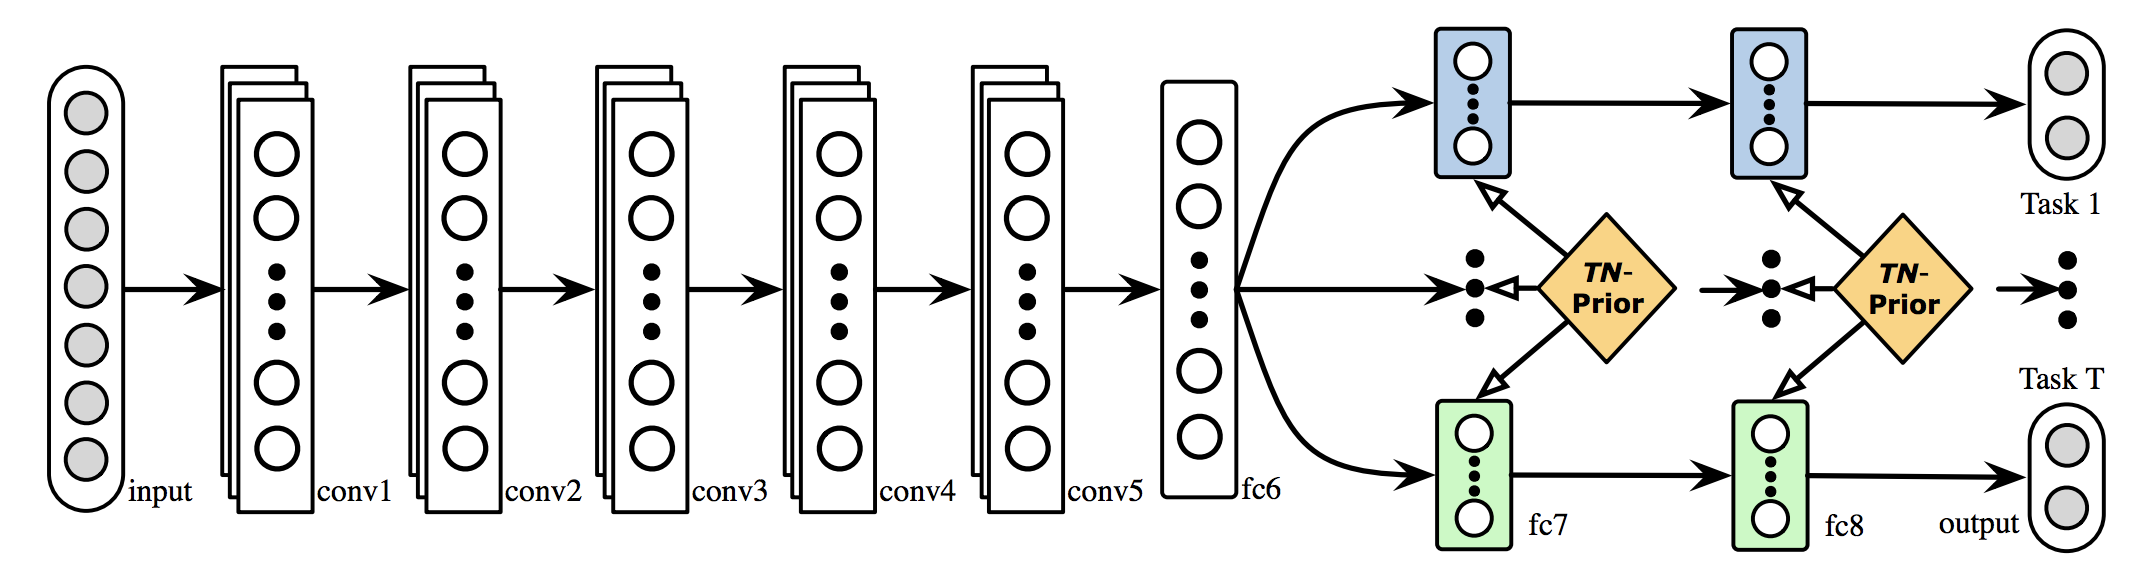
\includegraphics[scale=0.32,trim={0mm 0mm 0mm 0mm},clip]{long2017learning.png}
\end{figure*}

\begin{figure*}[t!]
	\centering
	\begin{subfigure}[b]{.65\linewidth}
		\centering
		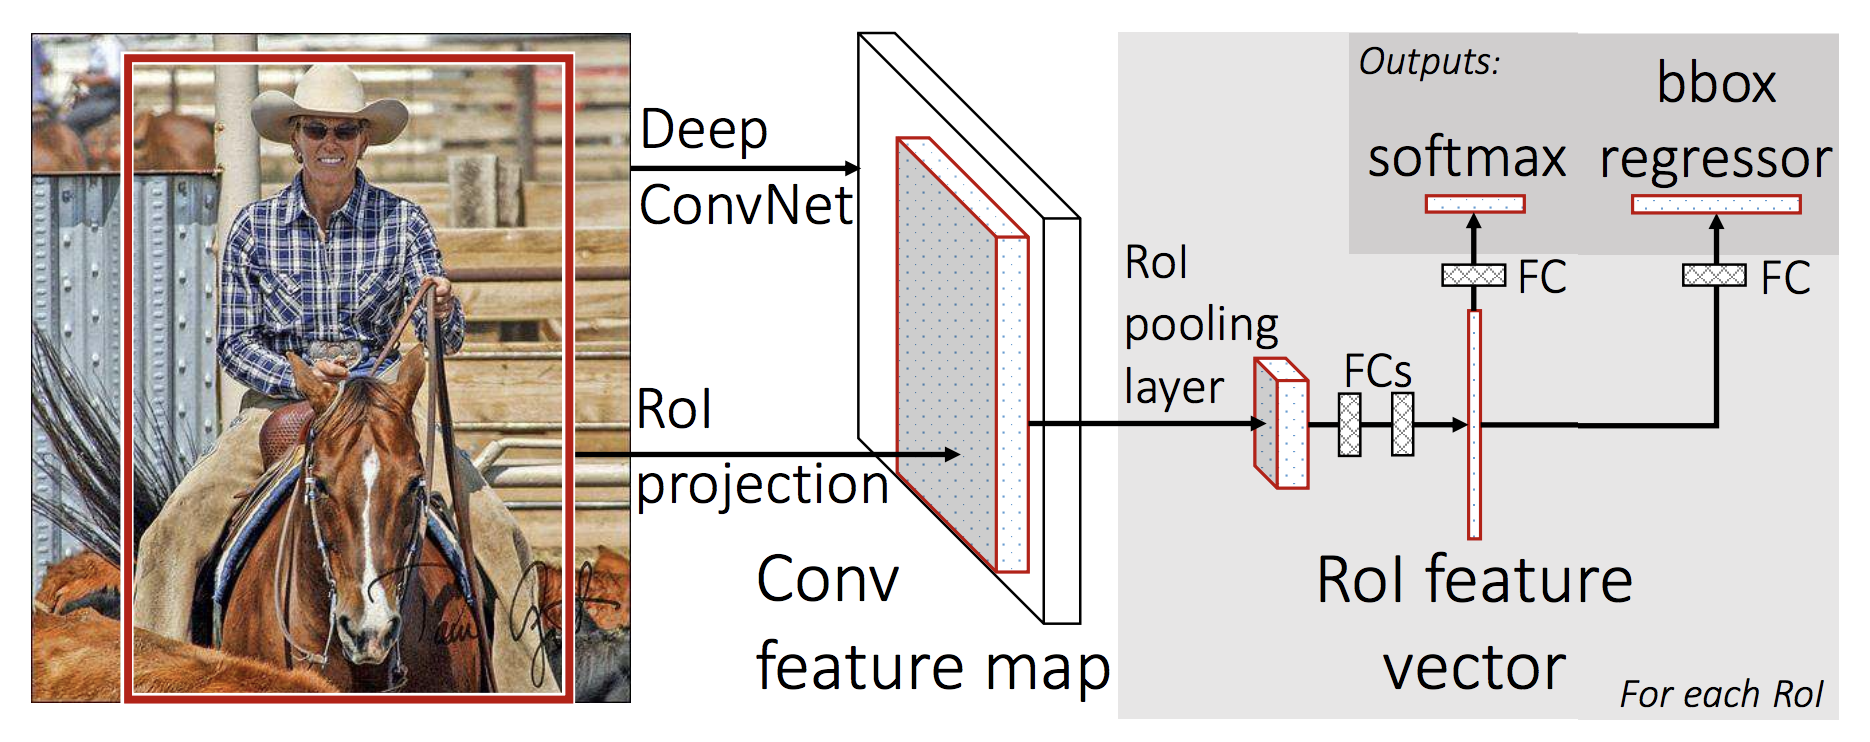
\includegraphics[scale=0.25,trim={0mm 0mm 0mm 0mm},clip]{girshick2015fast.png}
	\end{subfigure}%
	\begin{subfigure}[b]{.35\linewidth}
		\centering
		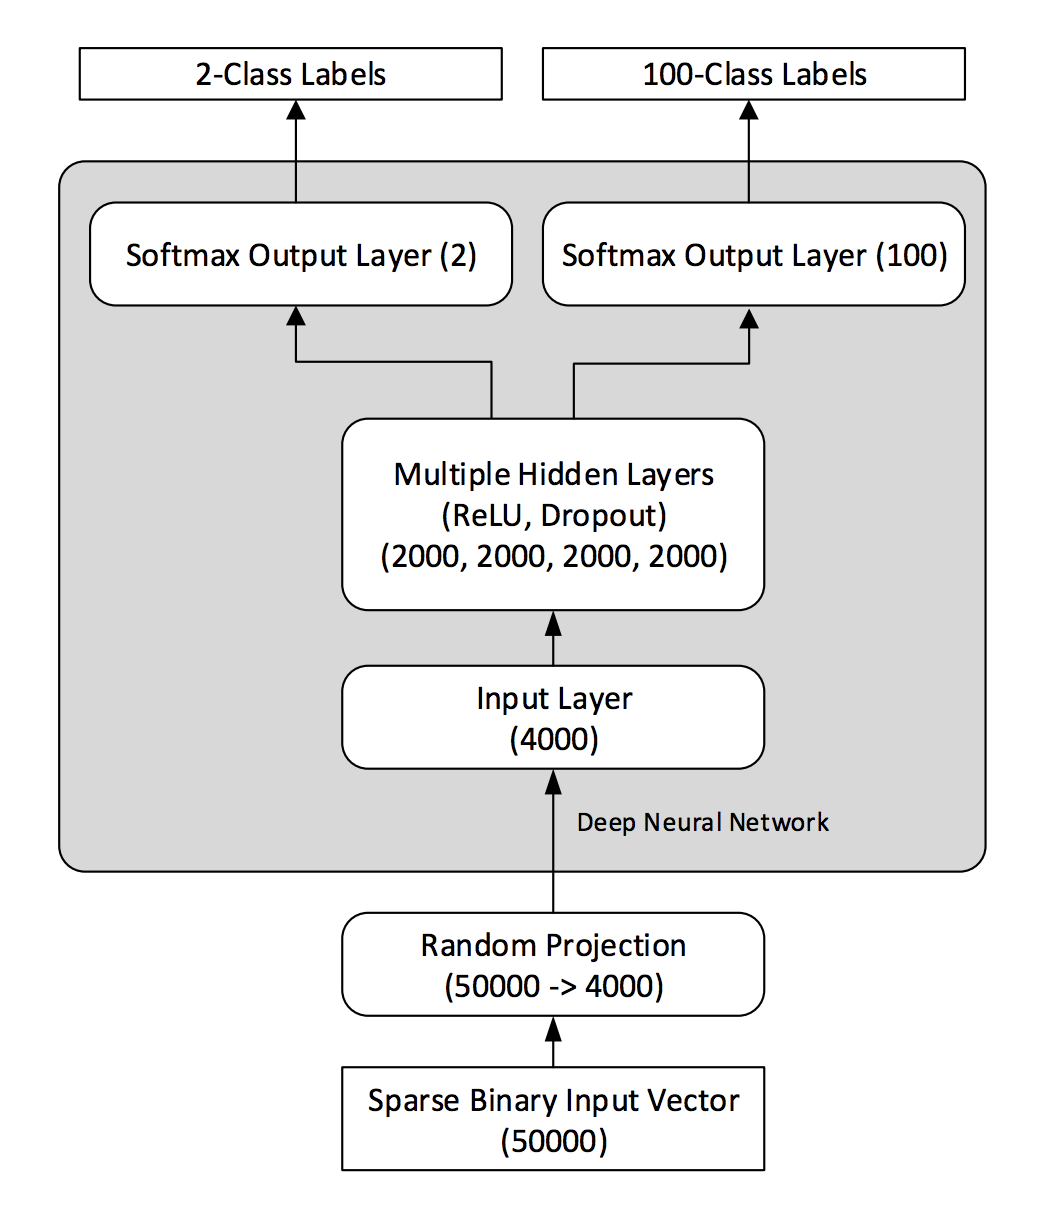
\includegraphics[scale=0.15,trim={0mm 0mm 0mm 0mm},clip]{huang2016mtnet.png}
	\end{subfigure}
	\caption{Model architectures proposed by ~\cite{long2017learning} (top), ~\cite{huang2016mtnet} (bottom right), and  ~\cite{girshick2015fast} (bottom left); Their approach for multi-task learning is to assign distinct fully-connected layer for each task.}
	\label{figure:mutli-task-learning}
\end{figure*}

One of the common approach for multi-task learning is to assign distinct fully-connected layer for each task (see Figure~\ref{figure:mutli-task-learning}). With such architecture, each task is trained independently while weights for upstream layers are shared among tasks. Once the training completes for the combined model, a task can be discarded from populating output by removing corresponding fully-connected layer.

Next, consider a case of transfer learning. It is found that pre-training a model and fine-tuning the model for target task can leads to increase in accuracy. There is no change in model architecture throughout this process. Therefore, fine-tuned model uses the same amount of computation as the model that is explicitly trained to accomplish the same task.

Recall the criteria for dynamic model construction. Above multi-task learning approach achieves the dynamic addition and removal of a class and transfer learning guarantees the necessary efficiency. Exploiting these two techniques in two different domains, the proposed algorithm has the following step:

\begin{enumerate}
    \item Pre-train a model as if it is multi-classification problem
    \item Freeze the model parameters
    \item Repeat step 4 $\sim$ 7 for each class
    \item Construct a dataset which labels target class as positive and the others as negative.
    \item Replace the last full-connected layer for two classes
    \item Fine-tune the last layer using the new dataset
    \item Retrieve class-specific weights (weights for positive class) of the fully-connected layer
    \item For every variation of target set, it is possible to construct corresponding model by replacing the last layer with the class-specific weights obtained from fine-tuning.
\end{enumerate}

For simplicity, I decide to call this algorithm as Composing algorithm, the model trained for multi-class as base model, models constructed from step 4 $\sim$ 7 as fine-tuned models and the model constructed from the last step as composed model.

Composing algorithm achieves dynamic addition and removal of a class by attaching and discarding corresponding fully-connected connections.
With such flexibility, retraining a classifier is no longer necessary. Furthermore, note that even though a class has not participated for step 1, it is possible to construct a composed model with that class as long as the same base model is used for fine-tuning.

When we are constructing a composed model, we only retrieve weights for positive class from each of fine-tuned model. Therefore, the composed model has exactly the same number of parameters with the base model. As a result, composing model does not violate the efficiency requirements.

\section{Accuracy Preservation}

However, does Composing algorithm also guarantees the accuracy requirements? To answer this question, we need to understand how different loss function affects the behaviour of the composed model.

\subsection{Limitations with cross entropy loss}

State of the art loss for multi-classification problem is cross entropy (CE) loss, which transforms output using softmax and calculates loss using negative log likelihood (NLL).
Softmax and NLL loss are defined as following:

\begin{align*}
Softmax(y_i) &= \frac{e^{y_i}}{\sum_{j}e^{y_j}} \\
NegativeLogLikelihood(y, t) & = -\frac{1}{N}\sum_{i=1}^N \left[ t_i \cdot \log y_i\right] \\
\end{align*}

where $x$ is the output of the network and $t$ is the target. target is one hot encoded vector as in common classification problem.

Softmax is normalized logits computed from the output of the network. Therefore each index has value between zero and one and sum is designed to be one. Since multi-class classifier rely on the mutually exclusive assumption with about the classes, CE loss is the most suitable as it promotes the positive class while suppressing the negative classes.

However, such assumption does not hold for composed model and CE loss can cause indeterministic behaviour with composed model. When CE loss is used throughout the composing algorithm, the loss which used in fine-tuning is computed with respect to the output of negative class. However, for a composed model, it is not fair to select the class with the greatest value as final class because model outputs for each class are not constructed with respect to each other.

For example, let us say there are 3 classes: A, B, and C. For fine-tuning, we construct a dataset which has two classes: one for target class (positive class) and the other constructed with the other two classes (negative class). Once models are fine-tuned for each class, we have weights for positive class and negative class. For simplicity, positive weights are referred with lower case (a, b, and c) and negative weights with lower case with prime (a', b', and c'). During fine-tuning, loss is calculated in pairs: a -- a', b -- b', c -- c'. However, when we construct a composed model, the last layer consists of weights a, b and c. As a results, selecting the highest value as a final class is not a valid approach.

\subsection{Binary cross entropy with sigmoid}

We now understand the limitation of CE loss caused by mutually exclusive assumption among classes. To overcome such issue, I propose binary cross entropy (BCE) loss with sigmoid.

\begin{align*}
Sigmoid(y_i) &= \frac{1}{1 + e^{-x_i}} \\
BinaryCrossEntropy(y, t) & = -\frac{1}{N}\sum_{i=1}^N \left[ t_i \cdot \log y_i + (1 - t_i) \cdot \log (1 - t_i) \right] \\
\end{align*}

Unlike softmax in CE Loss, the only input for sigmoid is the output from the network at the corresponding index. Furthermore, while CE loss considers mutually exclusive assumption as part of its calculation, BCE loss considers each index independently and is calculated with respect to its target. As a result, weights for each class in fine-tuned model no longer depend on other factors. This indicates that class with the highest output from composed model has the highest probability of being true class.

It is found that multi-label classification has raised the same issue with CE loss~\cite{liu2017deep}. It is found that the independence guarantee provided by BCE loss with sigmoid is crucial for multi-label classification and enabled successful training of a model.

\section{Experiments}

Realising the theoritical limitation of cross entropy loss, I have conducted thorough experiments using PyTorch, reporting how different loss function affects the performance of composed model.

In this experiment, I evaluate three different loss functions. First loss function is CE loss. Since PyTorch NLL loss implementation expects log probability, log is applied after softmax but it is found that this does not affect the conclusion from the experiments. Next, I include sigmoid with BCE loss which successfully preserves accuracy between base and composed model. Lastly, I include BCE loss with softmax. This setting is known to be unstable because BCE loss assumes the independence among classes. In fact, I have observed the training collapse once it reaches a certain point. However, since we report accuracy from the best model, results from this setting is still valid and meaningful. This setting should demonstrate how crucial sigmoid is in the composing algorithm as it simply replace sigmoid with softmax from last setting.

Experiments are conducted with MNIST, Keyword Spotting, and CIFAR100 varying on number of classes, 10, 30, and, 100 respectively. From each experiment, I report accuracy of base model, fine-tuned model, and composed model. Furthermore, as I construct composed model by adding a class at a time, I also report accuracy for each intermediary composed model to understand how how number of classes affects the accuracy of combined model. It is found that the intermediary composed model accuracy fluctuate quite a bit depending on the order each class is added. Therefore, I repeat this process 10 times for each base model as I randomly select a class to add next.

\subsection{MNIST}

MNIST is a standard benchmark for classification~\cite{lecun1998gradient} which consist of images for handwritten digits. Among the wide range of model architecture solving this problem, I have conducted my experiments with \texttt{LeNet-5} ~\cite{lecun2015lenet}. \texttt{LeNet-5} is constructed with two convolutional, one dropout and two fully connected layers. The original implementation of \texttt{LeNet-5} has 10 and 20 channels for the two convolutional layers and produces accuracy of 98\% on MNIST dataset. Since our goal of this experiment is to understand the difference in peformance caused by different loss functions, I intentionally limited the expressive power of the network by constructing the network with only 5 channels for both convolutional layers.

Both base model training and fine-tuning is conducted using Adam optimizer with learning rate of 0.0001. After conducting 50 iterations of the experiment, it is found that all three loss function converges to similar accuracy within 5 epochs. The base models converge to average accuracy of 95\% and fine-tuned models converge to 98\% (see Figure \ref{table:mnist}).

Table \ref{figure:composed_mnist} summarizes how the accuracy changes as number of classes increases for composed model. No matter which loss function is used for composing algorithm, decrease in accuracy is found as more classes are involved for the composed model construction. However, models with softmax based loss is found to suffer at a greater rate than models with sigmoid based loss. With CE loss, the composed model for all 10 classes has an accuracy of 85.86\% introducing 10.5\% decrease with respect to the base model. decrease from BCE loss with softmax is found to be the greatest as the accuracy decreases by 17.85\% with the final accuracy of 78.50\%. On the other hand, BCE loss with sigmoid introduces the minimal degradation of 0.2\% and achieves the final accuracy of 95.29\%. \red{This proves that class independence training is crucial with the composing algorithm.}

\begin{table}[t]
    \centering
    \begin{tabular}{ccccccc}
        \toprule[1pt]
        \multirow{2}{*}{\raisebox{-3\heavyrulewidth}{\bf Loss function}} &
        \multirow{2}{*}{\raisebox{-3\heavyrulewidth}{\bf Base model}} &
        \multicolumn{3}{c}{\bf Fine tuned model } &
        \multicolumn{2}{c}{\bf Composed model } \\
        \cmidrule(lr){3-5}
        \cmidrule(lr){6-7}
        & & average & minimum & maximum & accuracy & decrease rate \\
        \midrule
        LogSoftmax + NLL & 95.8 & 98.02 & 96.29 & 99.24 & 85.74 & 10.50 \\
        Softmax + BCE & 94.71 & 97.33 & 95.08 & 99.06 & 77.80 & 17.85 \\
        Sigmoid + BCE & 95.49 & 98.07 & 96.74 & 99.19 & 95.30 & 0.20 \\
        \bottomrule[1pt]
    \end{tabular}
    \caption{Average accuracy of base, fine-tuned, and composed model for MNIST}
    \label{table:mnist}
\end{table}

\begin{figure}[t]
    \centering
    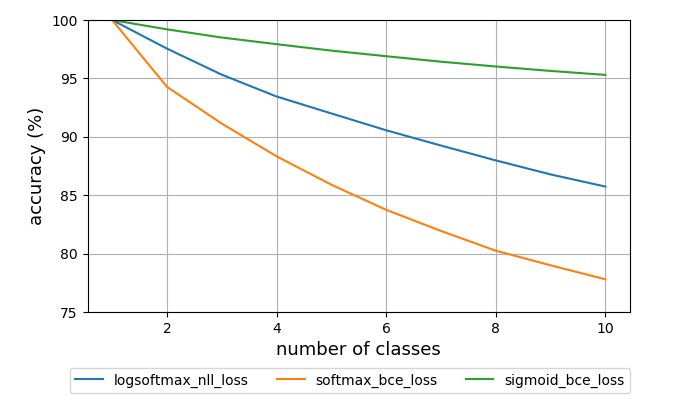
\includegraphics[scale=0.5,trim={0mm 0mm 0mm 0mm},clip]{mnist.png}
    \caption{Accuracy of composed model for MNIST with respect to number of classes}
    \label{figure:composed_mnist}
\end{figure}

\subsection{Keyword Spotting}

In order to evaluate the universality of composing algorithm, I extend the idea to keyword spotting where the input data is audio. The goal of Keyword Spotting (KWS) is to detect an audio of pre-trained keywords, such as “Hey Siri”. Since the first menaing results introduced by~\cite{chen2014small}, Neural network has been the {\it de facto} approach for KWS. In this experiment, I implement \texttt{res15-narrow} introduced by~\cite{tang2018deep}, which achieves accuracy of 94\% for 12 keywords on Google’s Speech Commands Dataset~\cite{speechcommandsdataset}. \texttt{res15-narrow} comprises 6 residual blocks with 19 feature maps where each residual block is composed of bias-free convolutional and batch normalization layer.

As opposed to the previous studies with Google’s Speech Commands Dataset where accuracy is evaluated on 12 keywords, I include all 30 keywords as I am interested in how stable the composing algorithm with respect to the increasing number of classes. Following the standard feature extraction process for audio, I first construct Forty-dimensional Mel-Frequency Cepstrum Coefficient (MFCC) frames and stack them using 30ms windows with a 10ms shift. Since the dataset has one-second long utterances of each word, the final processed input size is
$101\times40$.

Throughout 10 experiments conducted, stochastic gradient descent is used to train both base model and fine-tuned model with decreases in learning rate from 0.1 to 0.0001, stepping by a factor of ten. The base model is trained for 30 epochs with decrease in learning rate at 10 and 20 epochs. Unlike MNIST, the standard CE loss produces the best results; average accuracy of 93.11\%. It is found that the base model achieves average accuracy of 91.03\% and 89.63\% when trained using softmax with BCE loss and sigmoid with BCE loss respectively.

In order to obtain fine-tuned weights for each class, I further fine-tune the last fully-connected layer for 10 epochs with the decrease at 4 and 7 epochs. As summarized in table \ref{table:kws}, CE loss leads to the best fine-tuned models of 95.31\% accuracy. Similarly, softmax with BCE loss produces fine-tuned models with average accuracy of 91.84\% and sigmoid with BCE loss produces models with 91.28\%.

As observed in the experiment with MNIST, accuracy of composed model decreases as more classes are involved (see \ref{figure:composed_kws}. The model with CE loss shows the final accuracy of 90.24\% which is 3.08\% relative decrease from its base model accuracy. Softmax with BCE loss shows relative decrease of 4.09\% with the final accuracy of 87.31\% while the relative decrease in accuracy with sigmoid with BCE loss is only 1.62\% with the final accuracy of 88.18\%. Though composed model with CE loss demonstrates the best performance, sigmoid with BCE loss is found to be the most roboust loss function for composing algorithm with KWS.

\begin{table}[t]
    \centering
    \begin{tabular}{ccccccc}
        \toprule[1pt]
        \multirow{2}{*}{\raisebox{-3\heavyrulewidth}{\bf Loss function}} &
        \multirow{2}{*}{\raisebox{-3\heavyrulewidth}{\bf Base model}} &
        \multicolumn{3}{c}{\bf Fine tuned model } &
        \multicolumn{2}{c}{\bf Composed model } \\
        \cmidrule(lr){3-5}
        \cmidrule(lr){6-7}
        & & average & minimum & maximum & accuracy & decrease rate \\
        \midrule
        LogSoftmax + NLL & 93.11 & 95.31 & 92.89 & 97.17 & 90.24 & 3.08 \\
        Softmax + BCE & 91.03 & 91.98 & 89.29 & 95.28 & 87.31 & 4.09 \\
        Sigmoid + BCE & 89.63 & 91.28 & 89.08 & 93.97 & 88.18 & 1.62 \\
        \bottomrule[1pt]
    \end{tabular}
    \caption{Average accuracy of base, fine-tuned, and composed model for KWS}
    \label{table:kws}
\end{table}


\begin{figure}[t]
    \centering
    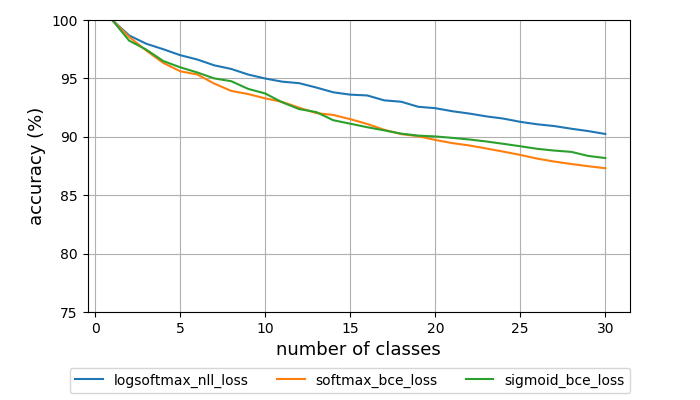
\includegraphics[scale=0.5,trim={0mm 0mm 0mm 0mm},clip]{kws.png}
    \caption{Accuracy of composed model for KWS with respect to number of classes}
    \label{figure:composed_kws}
\end{figure}

\subsection{CIFAR-100}

CIFAR is a collection of tiny colour images from the web introduced by~\cite{krizhevsky2009learning}. There exist two variations of CIFAR varying on number of classes: CIFAR-10 and CIFAR-100. The following experiment is constructed with CIFAR-100 which constitutes of 600 images of 100 classes.

For this experiment, I have implemented DenseNet, a state of the art model architecture for CIFAR dataset~\cite{huang2017densely}. Building upon the architecture with residual connection, the feature-maps of all preceding layers are used as inputs for each layer. Following the standard implementation introduced by~\cite{huang2017densely}, the network has three dense blocks with transition layers between which changes the feature-map sizes by convolution and pooling. I include results from two variations of DenseNet: \texttt{dense-40} and \texttt{dense-100} where each has 40 and 100 layers respectively.

\begin{table}[t]
    \centering
    \begin{tabular}{ccccccc}
        \toprule[1pt]
        \multirow{2}{*}{\raisebox{-3\heavyrulewidth}{\bf Loss function}} &
        \multirow{2}{*}{\raisebox{-3\heavyrulewidth}{\bf Base model}} &
        \multicolumn{3}{c}{\bf Fine tuned model } &
        \multicolumn{2}{c}{\bf Composed model } \\
        \cmidrule(lr){3-5}
        \cmidrule(lr){6-7}
        & & average & minimum & maximum & accuracy & decrease rate \\
        \midrule
        LogSoftmax + NLL & 93.11 & 95.31 & 92.89 & 97.17 & 90.24 & 3.08 \\
        Softmax + BCE & 91.03 & 91.98 & 89.29 & 95.28 & 87.31 & 4.09 \\
        Sigmoid + BCE & 89.63 & 91.28 & 89.08 & 93.97 & 88.18 & 1.62 \\
        \bottomrule[1pt]
    \end{tabular}
    \caption{Average accuracy of base, fine-tuned, and composed model for CIFAR-100}
    \label{table:cifar}
\end{table}


% \begin{figure}[t]
%     \centering
%     \includegraphics[scale=0.5,trim={0mm 0mm 0mm 0mm},clip]{cifar.png}
%     \caption{Accuracy of composed model for CIFAR-100 with respect to number of classes}
%     \label{figure:composed_cifar}
% \end{figure}


\section{Conclusion}
In this section please concisely describe what you are going to achieve in this project. E.g., formulate your problem precisely (mathematically), present the technical challenges (if any), discuss the tools or datasets that you will build on, state your goals, and come up with a plan for evaluation.

For your own sake, you might want to lay out a time line, so that you can keep a good track of your project.

\newpage

\section*{Acknowledgement}
Thank people who have helped or influenced you in this project.

\nocite{*}

\bibliographystyle{unsrtnat}
\bibliography{citation}

\end{document}
